\documentclass{source/Paper}
\usepackage{tikz}
% \usepackage{cite}
\usetikzlibrary{graphs, positioning, quotes, shapes.geometric}
\articletitle{``铝''途风云:铝材料与国家军事战略的核心关联}
\name{夏嘉彤}
\stuid{3240102804}
\Abstract{
    本文聚焦铝材料在军事战略领域的重要意义及其发展脉络。通过阐述铝材料从诞生到在一战、二战以及现代军事应用中的演变,深入分析其在航空、海军、陆军等多方面的应用实例,
    探讨技术革新对其性能提升的影响,
    揭示铝材料与国家军事战略之间的紧密关联,展现其在战争进程和军事发展进程中的关键作用。
}
\Keyword{铝材料;军事战略;战争应用;技术创新}
\engarticletitle{The Core Correlation between Aluminum Materials and National Military Strategy}
\engname{XIA Jia-tong}
\engKeyword{Aluminum Materials; Military Strategy; War Application; Technological Innovation}
\engAbstract{
    This article focuses on the significant importance of aluminum materials in the field of military strategy and its development context. By elaborating on the evolution of aluminum materials from their inception to their applications in World War I, World War II, and modern military scenarios, it conducts an in-depth analysis of application examples in various aspects such as aviation, navy, and army. It also explores the impact of technological innovation on the performance improvement of aluminum materials, reveals the close connection between aluminum materials and national military strategy, and demonstrates their crucial role in the process of war and military development.
}
\begin{document}
\maketitles
\newpage
\tableofcontents
\newpage
\setcounter{section}{-1}
\section{引言}
战争,作为人类社会矛盾的极端表现形式,始终是科技发展的强大驱动力。在众多在战争中发挥关键效能的材料里,铝以其独特的物理和化学特性,以及广泛的适用性,在军事领域中占据着不可替代的重要地位。从早期战争中的初步崭露头角,到现代战争中几乎无处不在的身影,铝材料犹如一颗璀璨的明星,见证并深刻塑造了战争的模式与走向。随着时代的发展和技术的不断迭代升级,
铝材料在当今军事战略格局中的意义愈发凸显,
其影响深远且广泛,涉及军事装备的各个层面以及战争的诸多环节。
\section{铝材料的诞生}
铝,尽管在现代日常生活中随处可见,但其发展历程却相对短暂。早在 1746 年,德国科学家波特运用明矾成功制得氧化铝,这一开创性的成果为后续铝的研究奠定了基础。然而,在随后的近百年间,科学家们面临着一个巨大的挑战 —— 如何从氧化铝中提取出铝单质并降低生产成本。由于铝具有较强的活泼性,在当时的技术条件下,提取单质铝的难度极大,这使得铝产品成为了极其稀有的物品,其价格甚至一度与黄金相媲美。直至 1886 年,美国的霍尔和法国的艾鲁特同时取得了一项具有里程碑意义的突破 —— 他们分别独立获得了用冰晶石 - 氧化铝熔盐电解方法制取金属铝的专利。这一重大发现为铝的大规模工业化生产开辟了道路,1888 年美国匹兹堡建立了第一家电解铝厂,
标志着铝生产进入了一个全新的阶段,
为铝材料在工业领域的广泛应用奠定了坚实的基础,也为其在军事领域的登场拉开了序幕。
\begin{figure}[htbp]
    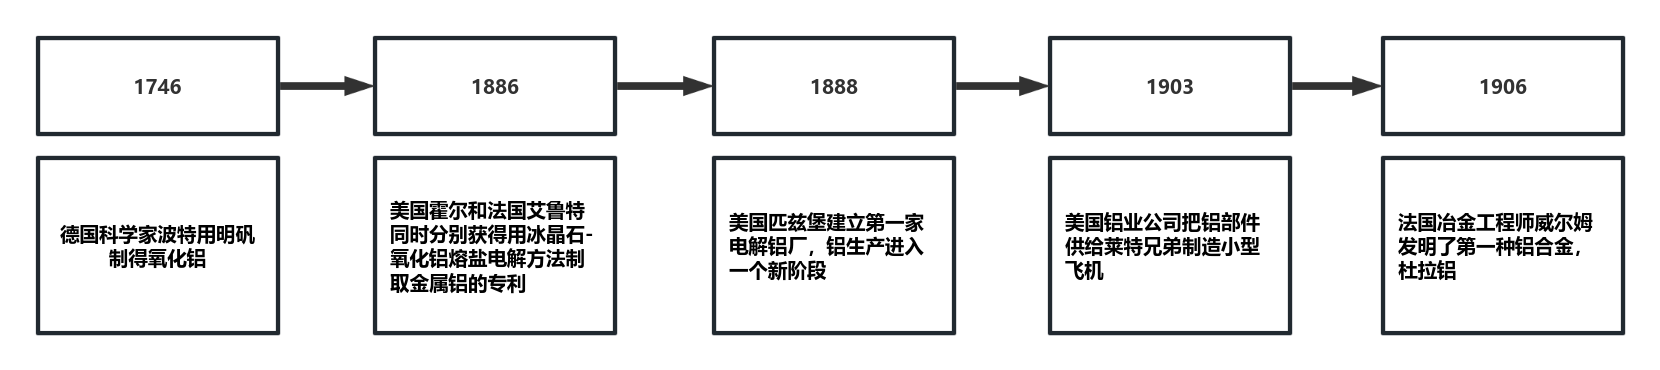
\includegraphics[width = 1\textwidth]{pic/图片1.png}
    \caption{铝材料的发展}
\end{figure}

\section{铝材料在一战中的应用}
第一次世界大战犹如一场巨大的风暴,席卷了整个世界,同时也为铝材料提供了一个崭露头角的广阔舞台。
在这一特殊的历史时期,军事需求呈现出爆发式增长,而铝材料凭借其独特的性能,迅速在军事领域找到了用武之地。
\subsection{航空领域的变革}
航空领域无疑是铝材料大放异彩的首个重要阵地。当时,飞机作为一种新兴的军事装备,正处于快速发展的关键阶段。传统的材料在满足飞机既要具备足够强度以承受飞行中的各种应力,又要尽可能轻便以提高飞行性能这一复杂需求上显得力不从心。而铝材料的特性恰好完美契合了飞机制造的这些严苛要求。各国纷纷开始广泛采用铝来制造飞机的机身框架、机翼等关键结构部件。轻巧的铝制飞机一经问世,便在军事航空领域展现出了巨大的优势。在起飞阶段,较轻的重量使得飞机能够更迅速地达到起飞所需的速度,缩短起飞滑跑距离,这在前线临时机场等条件有限的情况下尤为关键。在空中飞行操控方面,铝制飞机的灵活性和响应性得到显著提升,飞行员能够更加精准地驾驭飞机执行各种任务。更为重要的是,铝材料的应用使得飞机的航程大幅增加,能够覆盖更广阔的作战区域,同时载弹量也有了显著提升,从而大大增强了飞机的作战效能。铝制飞机的出现,彻底改变了空中作战的模式。从最初的侦察任务,到激烈的空中格斗,再到具有强大威慑力的轰炸行动,
铝制飞机将战争从传统的二维陆地和海洋空间延伸到了广阔的三维天空,开启了空战的新纪元,使天空成为了战争的又一重要战场。
\subsection{军事通信领域的助力}
除了航空领域,铝材料在军事通信领域也开始发挥重要作用。在战争中,高效、可靠的通信是军事指挥和协调作战的关键保障。铝材料因其良好的导电性和相对较轻的重量,被广泛用于制造通信设备的外壳和一些内部传导部件。这些铝制部件不仅保障了通信设备在复杂战场环境下的轻便性,便于士兵携带和快速部署,同时也确保了其具有足够的耐用性,能够在恶劣的气候条件、频繁的移动和可能的敌方攻击等情况下正常工作。通过使用铝材料,前线与后方之间的通信更加高效可靠,指挥官能够及时获取战场情报,准确下达作战指令,各作战部队之间也能够实现紧密的协同作战,从而极大地提高了军队的整体作战效能。
\subsection{军事运输工具中的应用}
在一些轻便型的军事装备运输工具中,铝材料也得到了一定程度的应用。例如,在轻型卡车、摩托车等运输车辆的制造中,部分零部件采用铝材料能够有效减轻车辆的整体重量。这不仅有助于提升运输效率,使车辆能够在相同的动力条件下更快地行驶,更重要的是能够保障战争物资的及时供应。在战争时期,快速、高效的物资运输对于维持军队的战斗力至关重要。铝材料的应用使得运输工具能够更灵活地穿梭于复杂的战场环境中,将弹药、食品、医疗物资等及时运送到前线部队手中,为战争的胜利提供了坚实的后勤保障。
\subsection{爆破性武器中的运用}
铝的特殊活泼性还使其在爆破性武器中得到了充分的运用。
早在一战时期,铝热剂(Thermite)燃烧弹就被投入到战争中,
并成为一种极具攻击性的武器。这种燃烧弹一般采用空中投放的方式,
既可以由飞行器载入空中投放,也可以在地面将其作为炮弹射入空中爆炸。
每发铝热剂燃烧弹通常装有十几个铝热剂填充罐,充足的反应材料确保了其强大的杀伤力。当铝热剂燃烧弹在空中爆炸时,会释放出超高温的 “火花”,这些 “火花” 不但覆盖面积大,能够对大面积的目标造成破坏,而且具有很强的粘合性,一旦附着在目标上便难以清除,会持续燃烧并对目标造成严重的损毁。\cite{__2023}在一战的战场上,铝热剂燃烧弹给敌方的军事设施、装备和人员带来了巨大的威胁,成为了一种令人生畏的武器。
\section{铝材料在二战中的应用及对战争结果的影响}
第二次世界大战的战火燃遍全球,规模和激烈程度远超一战,铝材料在这场战争中的应用也得到了更为广泛和深入的拓展,其对战争的进程和结果产生了深远影响,甚至在一定程度上成为了决定战争胜负天平倾斜方向的关键因素之一。
\subsection{航空领域的高度依赖}
在航空领域,随着战争的不断推进,各国对飞机性能的要求越来越高。铝材料在这一时期的应用达到了新的高度,高性能铝合金被大量研发和广泛使用。战斗机作为空中作战的主力,其发动机部件需要承受高温高压的极端环境,铝合金凭借其优异的耐高温和高压性能,被广泛应用于战斗机发动机的制造中。这使得发动机在高负荷运转下能够保持可靠稳定的运行,为战斗机提供了更强大的动力,使其在空中格斗中具备更快的速度、更高的机动性和更强的爬升能力,从而在空战中占据优势。轰炸机方面,随着战争战略的发展,对远程轰炸能力的需求日益增长。铝材料的轻量化特性使得轰炸机的大型化发展成为可能,其巨大的机身结构大量采用铝来减轻重量,从而在不牺牲载弹量的前提下显著增加航程。例如著名的 B - 29 轰炸机(英文:B-29 Bomber,绰号:Superfortress,译文:超级空中堡垒),其大规模使用铝材料,实现了跨洋轰炸作战的能力,能够对敌方的军事工业基地、战略目标等实施远程精确打击,对敌方的战争潜力造成了沉重打击,极大地改变了战争的战略态势。
\subsection{海军舰艇与舰载机的创新应用}
在海军方面,铝材料在舰艇制造中也有了创新性的应用。尽管钢铁仍然是舰艇主体结构的主要材料,但在一些上层建筑和非关键受力部件中使用铝,有效地减轻了舰艇的重量。这一改进带来了诸多好处,较轻的舰艇在航行时受到的水阻力减小,从而提高了航行速度,使其能够更迅速地抵达作战海域。同时,舰艇的机动性也得到增强,在躲避敌方攻击、进行战术机动等方面更加灵活自如。此外,铝制舰载机的广泛应用进一步增强了海军的航空作战能力。舰载机可以从舰艇上起飞,对敌方舰艇、沿海目标等进行攻击,大大拓展了海军的作战范围,使海上作战的形式更加多样化,从传统的舰艇炮战发展到海空立体作战,提升了海军在现代战争中的战略地位。
\subsection{陆军装备的轻量化突破}
在陆军装备中,铝材料的应用为陆军作战带来了新的变革。轻型坦克和装甲车的部分部件开始采用铝材料制造,这些装备在保持一定防护能力的同时,因铝材料的使用而更加轻便灵活。在复杂地形的机动作战中,如山地、丛林等地形,轻型铝制装甲车辆能够迅速穿插于战场,快速转移阵地,为陆军的战术实施提供了更多可能性。它们可以利用自身的机动性实施突袭、迂回包抄等战术,有效地打击敌方目标,同时也能够在敌方火力攻击下更迅速地撤离危险区域,提高了陆军部队的生存能力和作战效能。
\subsection{太平洋战役中的铝材料影响}
以太平洋战役为例,铝材料对战争结果的走向有着重大影响。美国在一战期间,铝生产由企业垄断并主要用于出口欧洲及日本。二战时期,珍珠港事件是一个重要转折点,此后美国政府大力介入铝产业。一方面,美国通过一系列政策和措施大幅增加本国铝产量,以满足战争对铝材料的巨大需求。另一方面,美国果断掐断了对日本的铝供应,这一举措对日本的战争能力产生了严重的制约。从产量数据来看,1939 年美国的铝产量为 16.4 万吨,而到了 1944 年这一数字飙升至 125 万吨。随着铝产量的急剧增加,美国的飞机制造业迎来了飞速发展,其在整个工业中的排名从原来的第 41 位直接跃升至第一位。在整个战争期间,美国一共生产了近 30 万架各型飞机,这些飞机在太平洋战场上发挥了巨大作用,对日本形成了强大的空中优势。
\cite{bilibili}而日本由于地理自然条件的限制,是一个资源匮乏的岛国,国土面积仅有 27 万平方公里,矿产、油气等各类资源均极度匮乏,严格意义上讲根本不具备发展铝工业的基础条件。
\cite{nihon}在铝供应被切断后,日本的飞机生产受到严重影响,无法满足战争需求,空中力量逐渐被美国压制,在战争中陷入了极为被动的局面,最终对太平洋战役的结果产生了决定性的影响。
\section{铝材料在近期的发展和创新}
在现代科技日新月异的推动下,铝材料在军事领域展现出了持续不断的发展和创新活力,不断适应现代战争日益复杂和多样化的需求。
\subsection{高性能铝锂合金的崛起}
从材料性能提升的角度来看,新型铝锂合金成为了当前研究和应用的热点领域。铝锂合金在继承铝材料低密度优势的基础上,通过巧妙地添加锂元素,进一步优化了材料的微观结构,从而显著提高了材料的强度和刚度。在航空航天领域,新一代战斗机和航天器对材料性能提出了极高的要求,既要减轻重量以提高飞行性能和运载能力,又要具备足够的强度和刚度以承受高速飞行、复杂机动和恶劣太空环境带来的巨大应力。铝锂合金的出现恰好满足了这些需求,因此被大量应用于新一代战斗机的机身结构、机翼、起落架等关键部位,以及航天器的舱体、框架等部件。例如,先进战机在进行高机动飞行时,如高速俯冲、急剧拉升、大过载盘旋等动作时,机身会承受巨大的空气动力学压力,铝锂合金机身凭借其出色的强度和刚度,能够有效抵抗这些压力,确保飞机结构的完整性和安全性,保证飞行任务的顺利进行。在航天器领域,铝锂合金的应用使得航天器在减轻重量的同时,能够更好地抵御太空辐射、微流星体撞击等恶劣环境因素的影响,提高航天器的可靠性和使用寿命。
\subsection{先进加工工艺的突破}
在加工工艺方面,现代军事领域对铝材料零部件的精度和复杂性要求越来越高,先进的精密加工技术应运而生。这些技术能够将铝材料加工成各种形状复杂、精度极高的军事零部件。以导弹制导系统为例,导弹的精确制导依赖于高精度的零部件来实现准确的信号传输、姿态控制和飞行轨迹调整。通过高精度的加工工艺,可以将铝制部件加工到微米级甚至纳米级的精度,确保导弹在飞行过程中能够精确地感知目标信息,稳定地控制飞行姿态,从而实现对目标的精确打击。同时,3D 打印技术在铝材料军事应用中的尝试也为装备制造带来了全新的思路和方法。3D 打印技术具有高度的灵活性和定制化能力,能够根据设计要求快速制造出一些形状复杂、传统加工工艺难以实现的铝制零部件。这不仅大大缩短了装备研发周期,使新型军事装备能够更快地投入使用,而且提高了装备的定制化水平,能够根据不同的作战任务和战场需求,快速生产出具有针对性性能的零部件,提高了军队在复杂多变的战争环境中的应对能力。此外,在透明装甲领域,通过特殊加工工艺制作出的透明铝装甲展现出了卓越的性能。这种透明铝装甲由氮氧化铝(一种铝、氧、氮的化合物)制成,在透明度、密度和抗刮蹭性能上都远远优于传统透明装甲材料。它能够清晰地提供视野,同时又能有效抵御 12.7mm 穿甲弹和常用 7.62mm 防空武器的射击,为军事装备提供了可靠的防护,而其重量和厚度却仅为传统透明装甲的一半。
\cite{guard}这使得军事装备在保持防护性能的同时,能够减轻重量,提高机动性和灵活性。
\subsection{表面处理技术的革新}
铝材料的表面处理技术也取得了新的重大突破。在军事环境中,装备面临着各种恶劣条件的考验,如高温、高湿、高盐雾、强腐蚀等。通过特殊的涂层和表面处理方法,能够在铝材料表面形成一层具有优异性能的保护膜。这层保护膜可以有效地增强铝材料在恶劣环境下的耐腐蚀、耐高温和抗磨损能力。在军事装备长期储存过程中,表面处理后的铝材料能够抵御环境因素对其的侵蚀,保持良好的性能状态,减少因腐蚀、老化等原因导致的装备损坏和性能下降,从而延长装备的储存寿命。在复杂环境作战中,如沙漠、海洋、丛林等环境,经过表面处理的铝制装备能够更好地适应恶劣环境,减少维护保养的频率和难度,降低维护成本。这不仅提高了军事装备的使用效率和可靠性,也进一步巩固了铝材料在现代军事战略中的核心地位,使其在现代战争中能够持续发挥重要作用。
\section{结论}
铝材料自诞生以来,其发展历程与军事战略紧密交织。从一战中的初步应用到二战中的广泛拓展,再到现代的创新发展,铝材料在军事领域的地位不断攀升。其在航空、海军、陆军等多方面的应用实例充分展示了对战争模式、军事装备性能提升以及战争结果的深远影响。随着科技的持续进步,铝材料在性能提升、加工工艺改进和表面处理技术革新等方面不断取得新突破,将继续在军事领域发挥不可替代的关键作用。各国也必将更加重视铝材料的研发与应用,以在日益激烈的军事竞争中占据有利地位。同时,铝材料的发展也将持续推动军事战略的演变和调整,对未来战争格局产生更为深远和广泛的影响。在未来的军事发展进程中,铝材料有望继续书写其辉煌篇章,为国家安全和军事战略目标的实现贡献重要力量。

\bibliography{ref2}

\newpage
\appendix
\section{附-对课程的感想}
\subsection{写作感想}
在军理课之前,军事相关的知识和事件对我来说陌生且遥远。军理课论文题目推荐里有一项是从自己的专业角度,考察自己的专业和战争的关系。我就读的是材料科学与工程专业,记得在分流面试的时候我说人类文明的进步历程其实就是材料的发展史,材料的发展对历史的演进起到了关键性的作用。所以在选题时我在想对于战争来说,材料也是至关重要的。在查阅了众多文献后,我将材料的范围缩小至“铝”这一单一金属材料。

范围缩小意味着搜集资料的难度加大,中途有想过要再次放大主题,但是最终还是聚焦在铝上完成了相关阐述。

整个写作过程比较波折,同时也是收获满满。从一个材料的发展上逐渐了解百年来战争的情况,也体会到自己专业可以发挥出的价值。论文也许写得还很幼稚,但是过程中的收获比起结果更有价值。
\subsection{军理课的感想}
老师幽默风趣的语言带来的军事理论课为我打开了一扇洞察军事世界的新窗口,极大地拓宽了我的视野。虽然在军事理论方面我确实是小白,但是在具体而有趣的事例以及阐述清晰逻辑连贯的介绍中,我感觉到军事跟我的距离并不遥远。
\end{document}